\documentclass[a4paper,12pt]{article}
\usepackage{a4wide}
\usepackage{tikz}
\usetikzlibrary{calc}
\usepackage{hyperref}

\begin{document}
\pagestyle{empty}
\setlength{\parindent}{0em} 
\section*{ROM (Instruction Memory)}


Your task is to program the behavior of an entity called "ROM". This entity is declared in the attached file "ROM.vhdl" and has the following properties:
\begin{itemize}
\item Inputs: Clk and enable with type std\_logic; these are clock and enable signals
\item Inputs: addr with type std\_logic\_vector; the address of the instruction which is going to be read
\item Outputs: output with type std\_logic\_vector; this is the instruction which is read 
\end{itemize}
\vspace{0.3cm}
\begin{center}
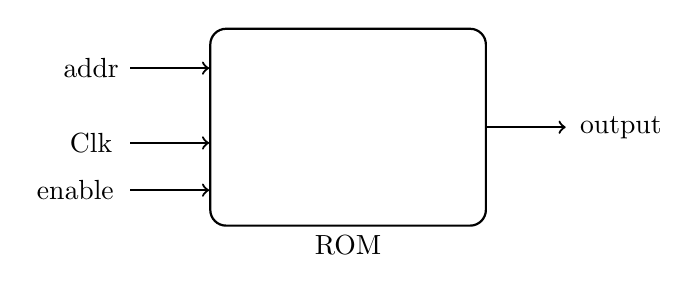
\begin{tikzpicture}
\draw node [draw,rectangle, minimum height=25mm, minimum width=35mm,rounded corners=2mm,thick](entity){};
\draw[->,thick] ($ (entity.west)-(10mm,-7.5mm)$) -- ($ (entity.west) - (0mm,-7.5mm)$);
\draw node at ($ (entity.west)-(15mm,-7.5mm)$){addr};
\draw[->,thick] ($ (entity.west)-(10mm,2mm)$) -- ($ (entity.west) - (0mm,2mm)$);
\draw node at ($ (entity.west)-(15mm,2mm)$){Clk};
\draw[->,thick] ($ (entity.west)-(10mm,8mm)$) -- ($ (entity.west) - (0mm,8mm)$);
\draw node at ($ (entity.west)-(17mm,8mm)$){enable};

\draw[->,thick] ($ (entity.east) + (0mm,0mm)$) -- ($ (entity.east) + (10mm,0mm)$);
\draw node at ($ (entity.east) + (17mm,0mm)$){output};



\draw node at ($ (entity) - (0,15mm)$){ROM};

\end{tikzpicture}
\end{center}

Do not change the file "ROM.vhdl".\\

The "ROM" entity shall behave according to the following:\\

It has three inputs which are address, clock and enable signals. The length of address is %%ADDRLENGTH bits, and the length of instruction is %%INSTRUCTIONLENGTH which is equal to the length of the output. \\

You need to write the VHDL code of ROM and fill it with the sample list of instructions as below. Write the instructions (binary codes below) from address %%START to address %%STOP in the same sequence as they are written here. \\
Instructions:
\begin{center}
%%DATA\newline
\end{center}

Note that:

\begin{itemize}
\item the content of other locations in the ROM is zero.
\item it should be implemented as a single cycle ROM.
\item it works on %%CLK of the clock signal.
\item when the ROM is disabled the output is zero. When it is enabled the instruction stored at the input address is output at the output. 
\end{itemize}

This behavior has to be programmed in the attached file "ROM\_beh.vhdl".\\

To turn in your solution, write an email to %%SUBMISSIONEMAIL with Subject "Result Task %%TASKNR" and attach your file "ROM\_beh.vhdl".

\vspace{0.7cm}

Good Luck and May the Force be with you.



\end{document}
